\section{GPRM}

\subsection{What is the GPRM}

The Glasgow Parallel Reduction Machine is a virtual machine framework for multi-core programming using a task-based approach. It allows the programmer to structure their programs as a seperation of task-code (written as C++ classes) and communication code. 

Communication code is currently written in a language called GPIR (Glasgow Parallel Intermediate Representation). 
GPIR code controls how tasks communicate with one another and whether groups
of tasks can be evaluated sequentially or in parallel.  GPIR code is compiled down further to GPRM byte-code which is evaluated by the GPRM virtual machine.

The GPRM uses task nodes which consists of a task kernel and a task manager.

Task code is represeted as a task kernel. A task kernel is a self contained unit, typically represented as a C++ class.
To create a task kernel, the C++ class needs to be in the \textit{GPRM::Kernel::namespace}.

Communication code is represented as a task manager. A task manager "co-ordinates" communication between one or more task kernels, and
is represented as a function which can be called from a C++ program.\cite{GPRM}


When building, the GPRM packages the Task Kernels with 
GPRM generic code into a library. During this process the compiler analyses all classes and methods in the
Task Kernels and maps them to numeric constants. This process allows GPIR code to call Task Kernels.
GPIR code is also compiled down to GPRM bytecode packaged into the library. A serial C++ program when compiled is then linked to
this library and a call to the GPRM's "run" method executes the GPRM bytecode. 

\newpage

\begin{figure}[ht]
\pdfimageresolution=110
\begin{center}
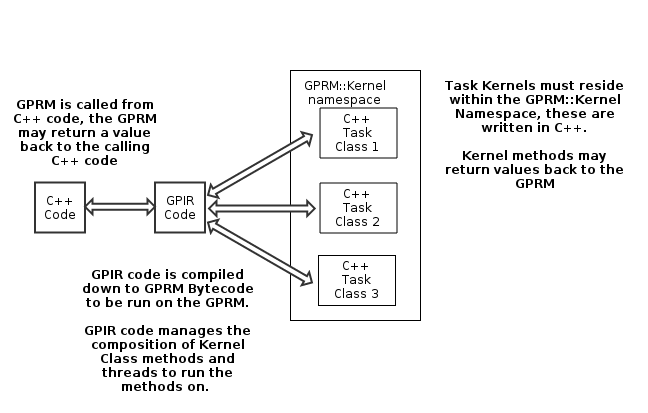
\includegraphics{graphs/gprm.png}
\caption{A simple overview of the GPRM framework}
\end{center}
\end{figure}

\subsection{The GPIR language}

The GPIR language is a purely functional S-expression based language that is evaluated in parallel by default 
with optional sequential evaluation semantics.

Tasks in GPIR are postifxed with a thread number to indicate to the GPRM runtime which thread
the task should run on. For example a simple GPIR program which adds numbers in parallel:

\begin{lstlisting}[style=myGPC]
(begin
    +[0] (+[0] '3 '2) (+[1] '4 '10)
)
\end{lstlisting}

The two nested additions are performed in parallel, with the first being mapped onto thread 0,
and the second being mapped onto thread 1. When they've both been evaluated, then the outer addition
will add the results on thread 0.

\subsubsection{Quoting}

Like in Scheme and Lisp, quoting an expression deffers the evaluation of it. 
This is useful for performing sequential evaluation.

\begin{lstlisting}[style=myGPC]
(seq 
    '(obj.m1[0] '1)
    '(obj.m2[0] '2)
)
\end{lstlisting}

Due to the parallel evaluation of GPIR, if the expressions in the seq block wern't quoted then
they would get evaluated in parallel instead of being deffered to be evaluated by the seq function.

Also literal values don't need to be evaluated, they should be deferred and passed to tasks which is
the reason the numbers are quoted in these examples.

\subsubsection{Registers}

The GPRM has registers which can be written to or read from.

\begin{lstlisting}[style=myGPIR]
(seq
    '(reg.write[0] '1 obj.m1[0])
    '(obj.m2[0] (reg.read[0] '1))
)
\end{lstlisting}

This program writes the result of the obj.m1 call to register 1,
then reads the result from register 1 and passed it into the obj.m2 call.

The GPIR language has other keywords and features but these are the ones that are important for
understanding the examples and design choices made for this project.
